\section{The Finite State Machine}
The FSM is the crux of interacting with the CAM and making it carry out complex arbitrary algorithms by exposing commands to carry out different tasks. 
It has numerous states, some of them are sending or receiving data, loading data into the CAM, selecting first, searching, reading, setting the comparand and mask as well as writing. 
The base UART module used is from David Things' Github repository. \cite{uart} This works on a 48MHz clock cycle.
To reduce complexities and avoid additional LUTs usage, we used the same clock speed throughout the project. 
\\\\
As shown in figure 4 (TODO), our FSM acts as a way to carry out procedural tasks while staying under the limit of 21 ns by linking states together. 
Therefore, a task may trigger several states before it returns to the default state. 
For example, the algorithm for searching has several steps, it comprises of
\begin{itemize}
    \item Setting the comparand 
    \item Setting the mask 
    \item Sending the SET signal 
    \item Sending the SEARCH signal 
\end{itemize}
Notice that the first two steps use several clock cycles as only one byte of data flows through the UART each clock cycle. 
This is due to its pipeline design. 
\\\\
The states transitions for the SET signal is given below:
\begin{itemize}
    \item  SET 1: change SET to high, set delay to 5 clock cycles
    \item  IDLE: wait for delay, go to SET 2
    \item  SET 2: change SET to low, listen for new command
\end{itemize}
In a very similar manner, all commands needed to operate a CAM were designed, these commands are triggered by sending a specific character to the CAM. 

\begin{{figure}
    \tikzset{every picture/.style={line width=0.75pt}} %set default line width to 0.75pt        

    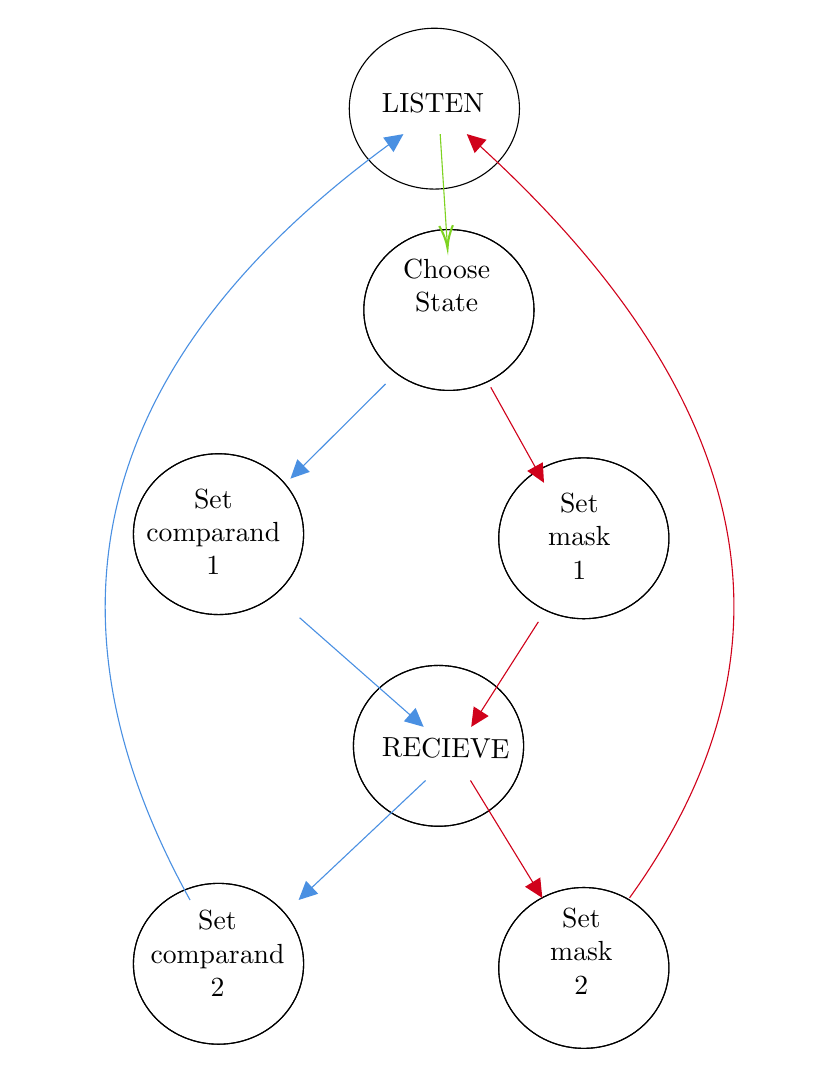
\begin{tikzpicture}[x=0.75pt,y=0.75pt,yscale=-1,xscale=1]
    %uncomment if require: \path (0,560); %set diagram left start at 0, and has height of 560

    %Shape: Ellipse [id:dp30119061586837703] 
    \draw   (123.23,354.75) .. controls (123.23,333.35) and (141.59,316) .. (164.23,316) .. controls (186.87,316) and (205.23,333.35) .. (205.23,354.75) .. controls (205.23,376.15) and (186.87,393.5) .. (164.23,393.5) .. controls (141.59,393.5) and (123.23,376.15) .. (123.23,354.75) -- cycle ;
    %Shape: Ellipse [id:dp4848885797268667] 
    \draw   (123.23,354.75) .. controls (123.23,333.35) and (141.59,316) .. (164.23,316) .. controls (186.87,316) and (205.23,333.35) .. (205.23,354.75) .. controls (205.23,376.15) and (186.87,393.5) .. (164.23,393.5) .. controls (141.59,393.5) and (123.23,376.15) .. (123.23,354.75) -- cycle ;
    %Shape: Ellipse [id:dp6948847640403879] 
    \draw   (17.23,252.75) .. controls (17.23,231.35) and (35.59,214) .. (58.23,214) .. controls (80.87,214) and (99.23,231.35) .. (99.23,252.75) .. controls (99.23,274.15) and (80.87,291.5) .. (58.23,291.5) .. controls (35.59,291.5) and (17.23,274.15) .. (17.23,252.75) -- cycle ;
    %Shape: Ellipse [id:dp2567147302347228] 
    \draw   (17.23,252.75) .. controls (17.23,231.35) and (35.59,214) .. (58.23,214) .. controls (80.87,214) and (99.23,231.35) .. (99.23,252.75) .. controls (99.23,274.15) and (80.87,291.5) .. (58.23,291.5) .. controls (35.59,291.5) and (17.23,274.15) .. (17.23,252.75) -- cycle ;
    %Shape: Ellipse [id:dp938096594364014] 
    \draw   (17.23,459.75) .. controls (17.23,438.35) and (35.59,421) .. (58.23,421) .. controls (80.87,421) and (99.23,438.35) .. (99.23,459.75) .. controls (99.23,481.15) and (80.87,498.5) .. (58.23,498.5) .. controls (35.59,498.5) and (17.23,481.15) .. (17.23,459.75) -- cycle ;
    %Shape: Ellipse [id:dp887993685343583] 
    \draw   (17.23,459.75) .. controls (17.23,438.35) and (35.59,421) .. (58.23,421) .. controls (80.87,421) and (99.23,438.35) .. (99.23,459.75) .. controls (99.23,481.15) and (80.87,498.5) .. (58.23,498.5) .. controls (35.59,498.5) and (17.23,481.15) .. (17.23,459.75) -- cycle ;
    %Shape: Ellipse [id:dp8591576771955458] 
    \draw   (128.23,144.75) .. controls (128.23,123.35) and (146.59,106) .. (169.23,106) .. controls (191.87,106) and (210.23,123.35) .. (210.23,144.75) .. controls (210.23,166.15) and (191.87,183.5) .. (169.23,183.5) .. controls (146.59,183.5) and (128.23,166.15) .. (128.23,144.75) -- cycle ;
    %Shape: Ellipse [id:dp42179166865495454] 
    \draw   (128.23,144.75) .. controls (128.23,123.35) and (146.59,106) .. (169.23,106) .. controls (191.87,106) and (210.23,123.35) .. (210.23,144.75) .. controls (210.23,166.15) and (191.87,183.5) .. (169.23,183.5) .. controls (146.59,183.5) and (128.23,166.15) .. (128.23,144.75) -- cycle ;
    %Shape: Path Data [id:dp8046463405438573] 
    \draw   (162.23,9) .. controls (184.87,9) and (203.23,26.35) .. (203.23,47.75) .. controls (203.23,69.15) and (184.87,86.5) .. (162.23,86.5) .. controls (139.59,86.5) and (121.23,69.15) .. (121.23,47.75) .. controls (121.23,26.35) and (139.59,9) .. (162.23,9) -- cycle ;
    %Shape: Ellipse [id:dp8077670693031269] 
    \draw   (193.23,254.75) .. controls (193.23,233.35) and (211.59,216) .. (234.23,216) .. controls (256.87,216) and (275.23,233.35) .. (275.23,254.75) .. controls (275.23,276.15) and (256.87,293.5) .. (234.23,293.5) .. controls (211.59,293.5) and (193.23,276.15) .. (193.23,254.75) -- cycle ;
    %Shape: Ellipse [id:dp29590588232724735] 
    \draw   (193.23,254.75) .. controls (193.23,233.35) and (211.59,216) .. (234.23,216) .. controls (256.87,216) and (275.23,233.35) .. (275.23,254.75) .. controls (275.23,276.15) and (256.87,293.5) .. (234.23,293.5) .. controls (211.59,293.5) and (193.23,276.15) .. (193.23,254.75) -- cycle ;
    %Shape: Ellipse [id:dp11804790571034007] 
    \draw   (193.23,461.75) .. controls (193.23,440.35) and (211.59,423) .. (234.23,423) .. controls (256.87,423) and (275.23,440.35) .. (275.23,461.75) .. controls (275.23,483.15) and (256.87,500.5) .. (234.23,500.5) .. controls (211.59,500.5) and (193.23,483.15) .. (193.23,461.75) -- cycle ;
    %Shape: Ellipse [id:dp29705692546094364] 
    \draw   (193.23,461.75) .. controls (193.23,440.35) and (211.59,423) .. (234.23,423) .. controls (256.87,423) and (275.23,440.35) .. (275.23,461.75) .. controls (275.23,483.15) and (256.87,500.5) .. (234.23,500.5) .. controls (211.59,500.5) and (193.23,483.15) .. (193.23,461.75) -- cycle ;

    % Text Node
    \draw (135.83,349.61) node [anchor=north west][inner sep=0.75pt]  [rotate=-0.67] [align=left] {RECIEVE};
    % Text Node
    \draw (16.73,230.01) node [anchor=north west][inner sep=0.75pt]   [align=left] {\begin{minipage}[lt]{56.588784000000004pt}\setlength\topsep{0pt}
    \begin{center}
    Set \\comparand \\1
    \end{center}

    \end{minipage}};
    % Text Node
    \draw (18.73,433.01) node [anchor=north west][inner sep=0.75pt]   [align=left] {\begin{minipage}[lt]{56.588784000000004pt}\setlength\topsep{0pt}
    \begin{center}
    Set \\comparand \\2
    \end{center}

    \end{minipage}};
    % Text Node
    \draw (139.73,119.01) node [anchor=north west][inner sep=0.75pt]   [align=left] {\begin{minipage}[lt]{40.715pt}\setlength\topsep{0pt}
    \begin{center}
    Choose \\State\\
    \end{center}

    \end{minipage}};
    % Text Node
    \draw (134.73,39.01) node [anchor=north west][inner sep=0.75pt]   [align=left] {\begin{minipage}[lt]{38.430608pt}\setlength\topsep{0pt}
    \begin{center}
    LISTEN
    \end{center}

    \end{minipage}};
    % Text Node
    \draw (212.73,232.01) node [anchor=north west][inner sep=0.75pt]   [align=left] {\begin{minipage}[lt]{27.093784000000003pt}\setlength\topsep{0pt}
    \begin{center}
    Set \\mask\\1
    \end{center}

    \end{minipage}};
    % Text Node
    \draw (213.73,432.01) node [anchor=north west][inner sep=0.75pt]   [align=left] {\begin{minipage}[lt]{27.093784000000003pt}\setlength\topsep{0pt}
    \begin{center}
    Set \\mask\\2
    \end{center}

    \end{minipage}};
    % Connection
    \draw [color={rgb, 255:red, 126; green, 211; blue, 33 }  ,draw opacity=1 ]   (165.03,60.01) -- (168.44,113.01) ;
    \draw [shift={(168.57,115.01)}, rotate = 266.32] [color={rgb, 255:red, 126; green, 211; blue, 33 }  ,draw opacity=1 ][line width=0.75]    (10.93,-3.29) .. controls (6.95,-1.4) and (3.31,-0.3) .. (0,0) .. controls (3.31,0.3) and (6.95,1.4) .. (10.93,3.29)   ;
    % Connection
    \draw [color={rgb, 255:red, 74; green, 144; blue, 226 }  ,draw opacity=1 ]   (138.73,180.37) -- (95.01,223.89) ;
    \draw [shift={(92.88,226.01)}, rotate = 315.13] [fill={rgb, 255:red, 74; green, 144; blue, 226 }  ,fill opacity=1 ][line width=0.08]  [draw opacity=0] (8.93,-4.29) -- (0,0) -- (8.93,4.29) -- cycle    ;
    % Connection
    \draw [color={rgb, 255:red, 74; green, 144; blue, 226 }  ,draw opacity=1 ]   (97.3,293.01) -- (154.81,343.62) ;
    \draw [shift={(157.06,345.6)}, rotate = 221.35] [fill={rgb, 255:red, 74; green, 144; blue, 226 }  ,fill opacity=1 ][line width=0.08]  [draw opacity=0] (8.93,-4.29) -- (0,0) -- (8.93,4.29) -- cycle    ;
    % Connection
    \draw [color={rgb, 255:red, 74; green, 144; blue, 226 }  ,draw opacity=1 ]   (158.01,371.42) -- (99.01,426.95) ;
    \draw [shift={(96.82,429.01)}, rotate = 316.74] [fill={rgb, 255:red, 74; green, 144; blue, 226 }  ,fill opacity=1 ][line width=0.08]  [draw opacity=0] (8.93,-4.29) -- (0,0) -- (8.93,4.29) -- cycle    ;
    % Connection
    \draw [color={rgb, 255:red, 208; green, 2; blue, 27 }  ,draw opacity=1 ]   (189.41,182.01) -- (213.59,225.39) ;
    \draw [shift={(215.05,228.01)}, rotate = 240.86] [fill={rgb, 255:red, 208; green, 2; blue, 27 }  ,fill opacity=1 ][line width=0.08]  [draw opacity=0] (8.93,-4.29) -- (0,0) -- (8.93,4.29) -- cycle    ;
    % Connection
    \draw [color={rgb, 255:red, 208; green, 2; blue, 27 }  ,draw opacity=1 ]   (256.24,428.01) .. controls (342.98,307.61) and (317.55,185.57) .. (179.92,61.87) ;
    \draw [shift={(177.84,60.01)}, rotate = 401.72] [fill={rgb, 255:red, 208; green, 2; blue, 27 }  ,fill opacity=1 ][line width=0.08]  [draw opacity=0] (8.93,-4.29) -- (0,0) -- (8.93,4.29) -- cycle    ;
    % Connection
    \draw [color={rgb, 255:red, 74; green, 144; blue, 226 }  ,draw opacity=1 ]   (44.51,429.01) .. controls (-33.45,288.05) and (0.1,165.57) .. (145.13,61.58) ;
    \draw [shift={(147.33,60.01)}, rotate = 504.61] [fill={rgb, 255:red, 74; green, 144; blue, 226 }  ,fill opacity=1 ][line width=0.08]  [draw opacity=0] (8.93,-4.29) -- (0,0) -- (8.93,4.29) -- cycle    ;
    % Connection
    \draw [color={rgb, 255:red, 208; green, 2; blue, 27 }  ,draw opacity=1 ]   (212.32,295.01) -- (181.6,343.07) ;
    \draw [shift={(179.98,345.6)}, rotate = 302.59000000000003] [fill={rgb, 255:red, 208; green, 2; blue, 27 }  ,fill opacity=1 ][line width=0.08]  [draw opacity=0] (8.93,-4.29) -- (0,0) -- (8.93,4.29) -- cycle    ;
    % Connection
    \draw [color={rgb, 255:red, 208; green, 2; blue, 27 }  ,draw opacity=1 ]   (179.62,371.42) -- (212.67,425.45) ;
    \draw [shift={(214.24,428.01)}, rotate = 238.55] [fill={rgb, 255:red, 208; green, 2; blue, 27 }  ,fill opacity=1 ][line width=0.08]  [draw opacity=0] (8.93,-4.29) -- (0,0) -- (8.93,4.29) -- cycle    ;

    \end{tikzpicture}
\end{figure}